%%
%% Copyright 2016 Dmitry Meshkov
%%

\documentclass[number,preprint,review]{elsarticle}

%% Use the options 1p,twocolumn; 3p; 3p,twocolumn; 5p; or 5p,twocolumn
%% for a journal layout:
%% \documentclass[final,1p,times]{elsarticle}
%% \documentclass[final,1p,times,twocolumn]{elsarticle}
%% \documentclass[final,3p,times]{elsarticle}
%% \documentclass[final,3p,times,twocolumn]{elsarticle}
%% \documentclass[final,5p,times]{elsarticle}
%% \documentclass[final,5p,times,twocolumn]{elsarticle}

%% For including figures, graphicx.sty has been loaded in
%% elsarticle.cls. If you prefer to use the old commands
%% please give \usepackage{epsfig}

%% The amssymb package provides various useful mathematical symbols
\usepackage{amssymb}
%% The amsthm package provides extended theorem environments
\usepackage{amsthm}
\usepackage{amsmath}

%% for url reference
\usepackage{hyperref}
\usepackage{graphicx}

%% The lineno packages adds line numbers. Start line numbering with
%% \begin{linenumbers}, end it with \end{linenumbers}. Or switch it on
%% for the whole article with \linenumbers.
%% \usepackage{lineno}
\def\infinity{\rotatebox{90}{8}}

\journal{??????????????????}

\begin{document}

\begin{frontmatter}

%% Title, authors and addresses

%% use the tnoteref command within \title for footnotes;
%% use the tnotetext command for theassociated footnote;
%% use the fnref command within \author or \address for footnotes;
%% use the fntext command for theassociated footnote;
%% use the corref command within \author for corresponding author footnotes;
%% use the cortext command for theassociated footnote;
%% use the ead command for the email address,
%% and the form \ead[url] for the home page:
%% \title{Title\tnoteref{label1}}
%% \tnotetext[label1]{}
%% \author{Name\corref{cor1}\fnref{label2}}
%% \ead{email address}
%% \ead[url]{home page}
%% \fntext[label2]{}
%% \cortext[cor1]{}
%% \address{Address\fnref{label3}}
%% \fntext[label3]{}

\title{Difficulty Control for Blockchain Systems}


%% use optional labels to link authors explicitly to addresses:
%% \author[label1,label2]{}
%% \address[label1]{}
%% \address[label2]{}

\author[iohk]{Dmitry Meshkov}
\ead{dmitry.meshkov@iohk.io}

\author[iohk]{Alexander Chepurnoy}
\address[iohk]{IOHK Research}

\begin{abstract}

The Bitcoin whitepaper~\cite{Nakamoto2008} states that the security of the system is guaranteed as long as honest miners control more than half of the current total computational power. In this paper we analyze a new way of attack on the blockchain based on mining difficulty manipulations. In spite of the fact that it does not allow to break blockchain security by double-spending, the attacker receive significant profit from this attack and average time interval between blocks increases as a side-effect. To reduce the attacker profit and to improve the stability of block times, we propose an alternative difficulty adjustment algorithm. The novel approach performs much better both in terms of block rate and in terms of attacker profit.

\end{abstract}

\begin{keyword}
Blockchain \sep Bitcoin \sep Decentralized consensus \sep Peer-to-peer networks \sep Proof-of-Work
\end{keyword}

\end{frontmatter}


\section{Introduction}
\label{sec:intro}

Blockchain systems have attracted a significant amount of interest from various communities after publication of Bitcoin whitepaper~\cite{Nakamoto2008} in 2008.
Bitcoin security relies on the distributed protocol that maintains the blockchain, called mining, in which network nodes tries to solve computational puzzle.
Other blockchain systems may rely on different computational puzzles~\cite{??} or even on virtual mining~\cite{??} while all of them use some algorithm that changes puzzle difficulty dynamically.
This algorithm for retargeting the difficulty is required to make blockchain system predictable and fix latency between blocks.

Fixed latency between blocks is important for several reasons.
Too frequent blocks leads to situation, when for a lot of miners block propagation time become bigger, then latency between blocks.
This leads to significant increasing of number of blockchain forks that complicates the consensus~\cite{decker2013information} and reduce effective hash rate in blockchain system.
On the other hand, increasing of the latency between blocks leads to decreasing of the network throughput~\cite{miller2016} and may be critical for high-loaded blockchain systems like bitcoin, where blocks are already 70\% full today~\cite{armstrong2016}.
Increasing latency by 50\% in bitcoin network will mean, that some transactions will be never included into blockchain.
Moreover this will lead to infinite growth of unconfirmed transactions pool, meaning it is likely that most bitcoin transactions will be not relayed.

Most of blockchain systems rely on difficulty retargeting algorithms assuming total computational power involved in mining process does not change over time.
Using more complicated retargeting algorithms with incorrect assumptions~\cite{andruiman2014} may lead to incorrect time interval between blocks even for simple case of constant hash rate as, for example, observed in Nxt, where observed mean time between blocks is ~2 times bigger, then expected in the whitepaper~\cite{nxt}. Moreover, too ofter difficulty recalculation leads to wide distribution of time intervals between blocks and makes blockchain system unpredictable~\cite{andruiman2014}.
Varying network computational power makes this algorithms inefficient for difficulty recalculation, e.g. continuous growth of computational power leads to decreasing mean latency between blocks and average block time in Bitcoin network is ~1.07 times lower, then expected.
Noteworthy, that exponential growth of computational power, which is the situation observed in practice in accordance with Moore’s law~\cite{moore2006cramming}, is the absolutely worst case (regarding the maximal block rate) possible for Bitcoin’s difficulty retargeting algorithm~\cite{kraft2015difficulty}.
On the other side, target recalculation algorithm should be simple enough and use integer arithmetic for all computational steps, since all nodes in the peer-to-peer network have to agree absolutely on the calculated difficulty.

Original Bitcoin white-paper, states that the security of the system is guaranteed as long as there is no attacker in possession of half or more of the total computational power used to maintain the system~\cite{Nakamoto2008}.
Most of the models used in the literature to discuss double-spending attacks assume that mining difficulty is constant~\cite{??}.
However difficulty is not constant, and can be manipulated by the attacker.
The Difficulty Raising Attack, introduced in~\cite{bahack2013theoretical}, enables the attacker to discard n-depth block, for any n and any attacker hash power, with probability 1 if he\footnote{For simplicity we choose to adapt the male form. This was chosen by flipping a coin.} is willing to wait enough time.
The fact that there is no way to determine whether a block have been computed on its declared time or not, have been used as part of other attacks~\cite{timejacking2011, artforz2011}.
In secton~\ref{sec:bit} we introduce a new attack for blockchain systems which manipulates difficulty for decreasing effective hash rate, required for block generation.

Novel studies of difficulty control proposes better functions for difficulty recalculation.
For example, the paper~\cite{kraft2015difficulty} introduces target recalculation function, designed to work “perfectly” not just for constant hash rate but also if the hash rate grows exponentially (with a constant but unknown rate).
Since it's good for situation, observed in practice in Bitcoin network, there are still a lot of open questions for future research.
Is it possible to create such a function, suitable for random fluctuations in the hash rate?
Is it possible to create such a function, simple enough to use integer arithmetic for all computational steps?
Is it possible to create such a function, stable for attackers manipulations?

\textbf{TODO transition to next section}

\section{Bitcoin Mining}
\label{sec:bit}

First, let us briefly describe how the mining process works.
The original concept is described in section 4 of the Bitcoin whitepaper~\cite{Nakamoto2008} and disscussed in plenty of papers~\cite{kraft2015difficulty, miller2014permacoin, eyal2014majority}.
We refer to the basic unit of mining work in Bitcoin as a scratch-off puzzle (SOP).
Miner generates candidates to the SOP by iterating thought \(nonse\) and calculating SHA-256 hash of a blocks header.
For a block to be valid it must value hash value less than the current \(target\) that is which is usually expressed in terms of the network difficulty \(D\) as \(1\over D\).
Thus, each hash attempt yields a valid block with probability \(1\over D\) and block frequency is \(R\over D\) where \(R\) is effective network hash rate.

Every \(M\) blocks (\(M=2016\) for Bitcoin) difficulty is recalculated as
\begin{equation}
D_{i+1}=D_i\cdot {MT\over S_m}
\end{equation}
where \(T\) is expected time interval between blocks and \(S_m\) is actual time, it took to generate \(M\) blocks.
Real time (\(~ 9 min 20 sec\)) interval is less, then desired time interval \(T=10 min\) because of continiuos growth of network computational power.
Difficulty recalculation interval \(M=2016\) has been chosen in such a way to recalculate difficulty every 2 weeks, while for real network it is a bit smaller.
This time intrerval is big enough to see increasing computational power of the network: right after target recalculation block time is close to desired 10 minutes, whereas at the end of \(epoch\) it's less then 9 minutes (see figure~\ref{fig:image}).
\begin{figure}[h]
\center{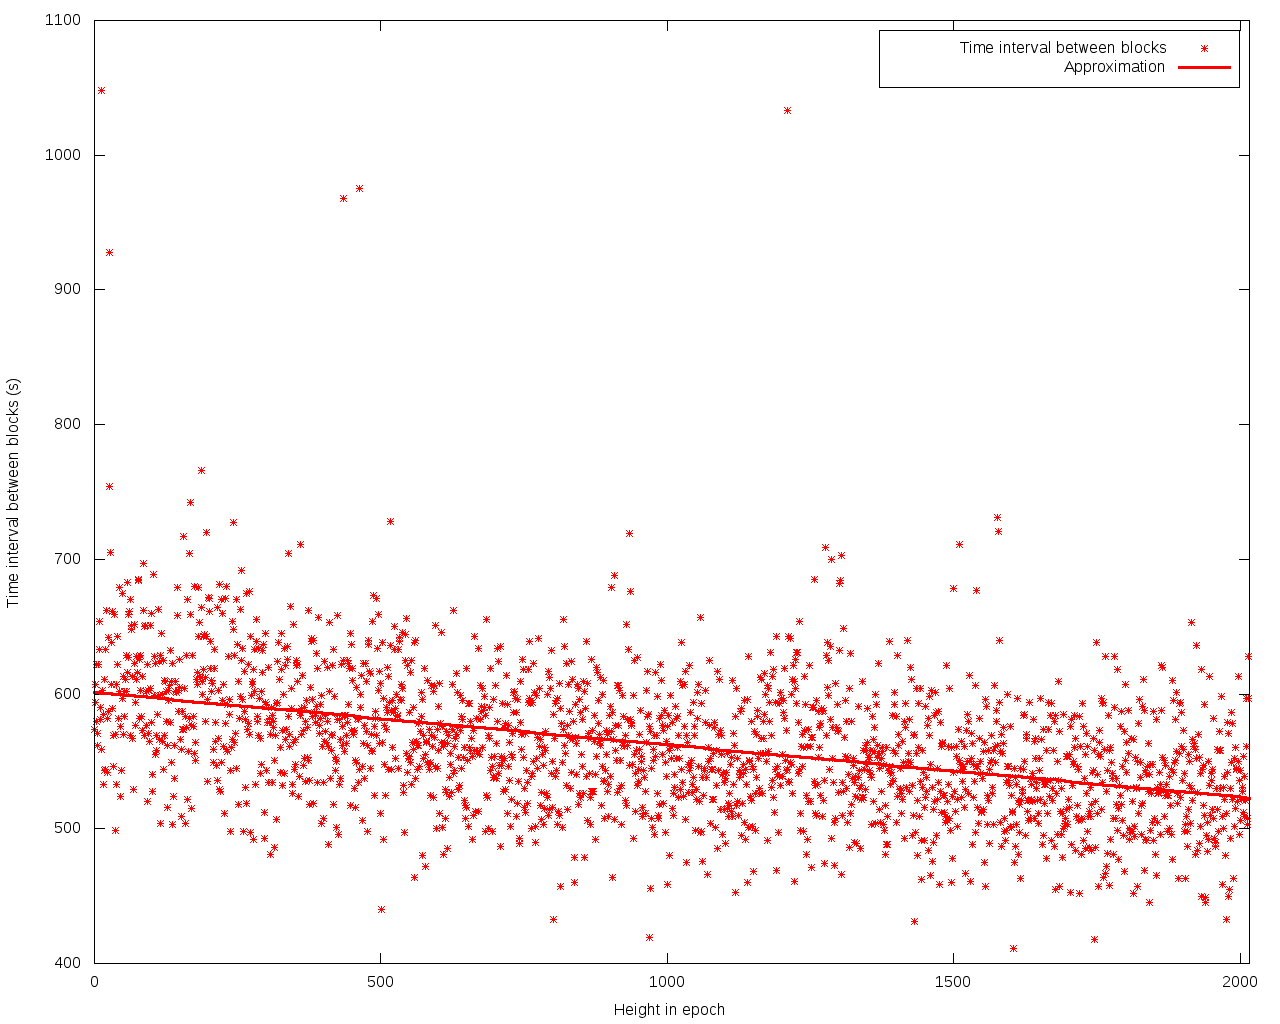
\includegraphics[scale=0.3]{interval.png}}
\caption{Average block time between difficulty recalculation}
\label{fig:image}
\end{figure}

\textbf{TODO transition to next section}

\section{Fork Switch Attack}
\label{sec:attack}

On this section we show a new way of manipulating difficulty with profit to an attacker.
The main idea is very simple.
The attacker may disable his mining, and wait for the next difficulty racalculation.
New difficulty will be lower, cause it don't include computational power of the attacker, and he turns on his mining again.
After next difficulty recalculation (which will include the attacker computational power) he turns off his mining again, and wait for next difficulty recalculation.
Such a simple algorithm allows him to mine during epochs with low difficulty, and don't mine during epoch with the low one, that will decrease computational resourses expended for block generation.
Of course in such a situation the attacker will create less blocks, that in situation, when he mine all the time.
However, lows of economy dictate that the cost of computational resourses invested into mining should be around the expected reward, and attackers profit, gained from every block may overbalance his wastes caused by decreasing number of created blocks.
Moreover, in a situation with a lot cryptocurency forks he is able to mine other forks in epoches with big difficulty and gain more blocks with more profit from each, that in situation, when he mine single cryptocurrency permanently.

 \textbf{TODO subsection?}

Let's calculate attacker profit in circumstances of Bitcoin difficulty recalculation function and constant hash rate (which is natural for this function).
Assume the situation when the network has some hash rate \(R_0\) provided by honest miners and the attacker has additional hash rate \(R_a=R_0\cdot p\) that it can turn on or off according to its purposes.
Usual miner with such a power will mine all the time with difficulty \(D_0=(R_0+R_a)\cdot T\) and will mine \(M\cdot R_a\over R_0+R_a\) blocks per epoch (\(M\) blocks) in average spending \(M\cdot R_a\cdot T\) computational power for them.
The attacker will start mining when difficulty \(D_0=R_0\cdot T\) is calculated from honest miners \(R_0\) only.
He will mine \(M\cdot R_a\over 2(R_0+R_a)\) blocks per epoch in average spending \(M\cdot T\cdot R_a\cdot R_0\over 2(R_0+R_a)\) computational power for them.
Consequently usual miner will spend \((R_0+R_a)T\) computational power per block, whereas attacker will just spend \(R_0T\) computational power per block.
The cost of computational resourses invested into mining should be around the expected reward.
If \(B\) is block reward and \(C\) is hash calculation cost, the usual miner profit is
\begin{equation}
{({M\cdot R_a\over R_0+R_a})\cdot B-M\cdot R_a\cdot T\cdot C=M\cdot R_a\cdot ({B\over R_0+R_a}-TC)}
\end{equation}
per epoch.
At the same time attackers profit is
\begin{equation}
{{M\cdot R_a \over 2\cdot (R_0+R_a)}\cdot (B - T\cdot R_0\cdot C)}
\end{equation}
and attack become profitable when
\begin{equation}
{{B\over C} < T\cdot (R_0+2\cdot R_a)}.
\end{equation}
Note, that if attacker is able to switch between different forks his epoch profit is twice bigger and is bigger then regular miner profit at any \(B\) and \(C\).


Remarkable, that under such an attack mean time between blocks will be
\begin{equation}
\label{eq:ati}
{T_a={T\over 2}({R_0+R_a\over R_0} + {R_0\over R_0+R_a})=T(1 + {p^2\over 2(1+p)})}
\end{equation}
which is strictly bigger then desired time \(T\).
Please notice that we regard \(p\) as the ratio between the hash-powers of the attacker and the honest network so it changes from 0 to \infinity.

\textbf{TODO transition to next section}

\section{An Improved Difficulty Control}
\label{sec:improved}

The difficulty-update algorithm employed by Bitcoin works as designed: If the hash rate is constant, it yields the desired block rate.
However it does not achieve the desired block rate in other situations and vulnerable to attack, described in \ref{sec:attack}.
In this section we are going to propose an alternative difficulty-update algorithm that works better, then Bitcoin's one.

First, we state properties of an \(ideal\) difficulty update algorithm:
\begin{enumerate}
\item{It should be resistant to known types of difficulty-update attacks.}
\item{It should lead to desired block rate for random fluctuations in the hash rate.}
\item{It should be simple enough to use integer arithmetic for all computational steps.}
\end{enumerate}
Security is the most important feature of blockchain systems and should be regarded with the highest priority.
Incorrect block rate is not considered a big problem in the Bitcoin community, but it may be important for more advanced applications of blockchain systems.
Implementation of the \(ideal\) difficulty update algorithm in subclass of integer programming is desired for different platforms compatibility.
This rule is not required, because, as mentioned in \cite{kraft2015difficulty}, it is possible to include non-integer algorithm parameters as part of the block, but it provides another way of difficulty manipulating to an attacker.

In this section we are going to regard difficulty update algorithm, based on well-knowen linear least squares method\cite{lawson1974solving}.
In the simpliest case of pair linear regression (\(y=kx+b)\) it's coefficients may be calculated as follows:

\begin{equation}
  \begin{cases}
    k= {{\overline{xy} - \overline{x}\overline{y}} \over {\overline{x^2} - \overline{x}^2}}  \\
    b=\overline{y}-k\overline{x}
  \end{cases}
\end{equation}
Note, that for accurate difficulty prediction we should use few last observed difficulties, rather than only one, as implemented in Bitcoin, but it's possible to use this algorithm right after second epoch.


We regard it as the good candidate for difficulty update algorithm, because:
\begin{enumerate}
\item{It should reduce profit of the attack, described in Section~\ref{sec:attack}.
Calculations of the attacker profit are described is Section~\ref{sec:sim}}
\item{It leads to desired block rate for linear changes in the hash rate.
This means, that regarding block rate, linear algorithm is better, then Bitcoin's one, in all cases, except constant hash rate, when they lead to the same result. }
\item{It is simple enough to use integer arithmetic for all computational steps with high fidelity.}
\end{enumerate}

\section{Simulations}
\label{sec:sim}

Finally, we want to present simulation results that show how our method proposed in Section~\ref{sec:improved} improves over Bitcoin’s difficulty update algorithm.
We'll regard \(difficulty\) growth in this section, keeping in mind the fact, that it's closely related with network hash rate, which is usually considered in literature.
All calculations have been performed with open-sourced programs, avaliable at Scorex project GitHub page~\cite{scorex}.

\textbf{TODO Linear?}

\subsection{Exponential Difficulty}

First let us regard exponential difficulty growth, wich is the situation observed in practice in Bitcoin network.
As we already mentioned, exponential difficulty growth is the absolutely worst case possible for Bitcoin’s difficulty retargeting algorithm.
For simplicity we regard a situation, when hash rate growth 10\% each epoch, more complicated research of exponential difficulty growth can be found in~\cite{kraft2015difficulty}.
Figure~\ref{fig:exp} presents difficulty as the function of epcoh, which is 2016 blocks in Bitcoin.

\begin{figure}[h]
\center{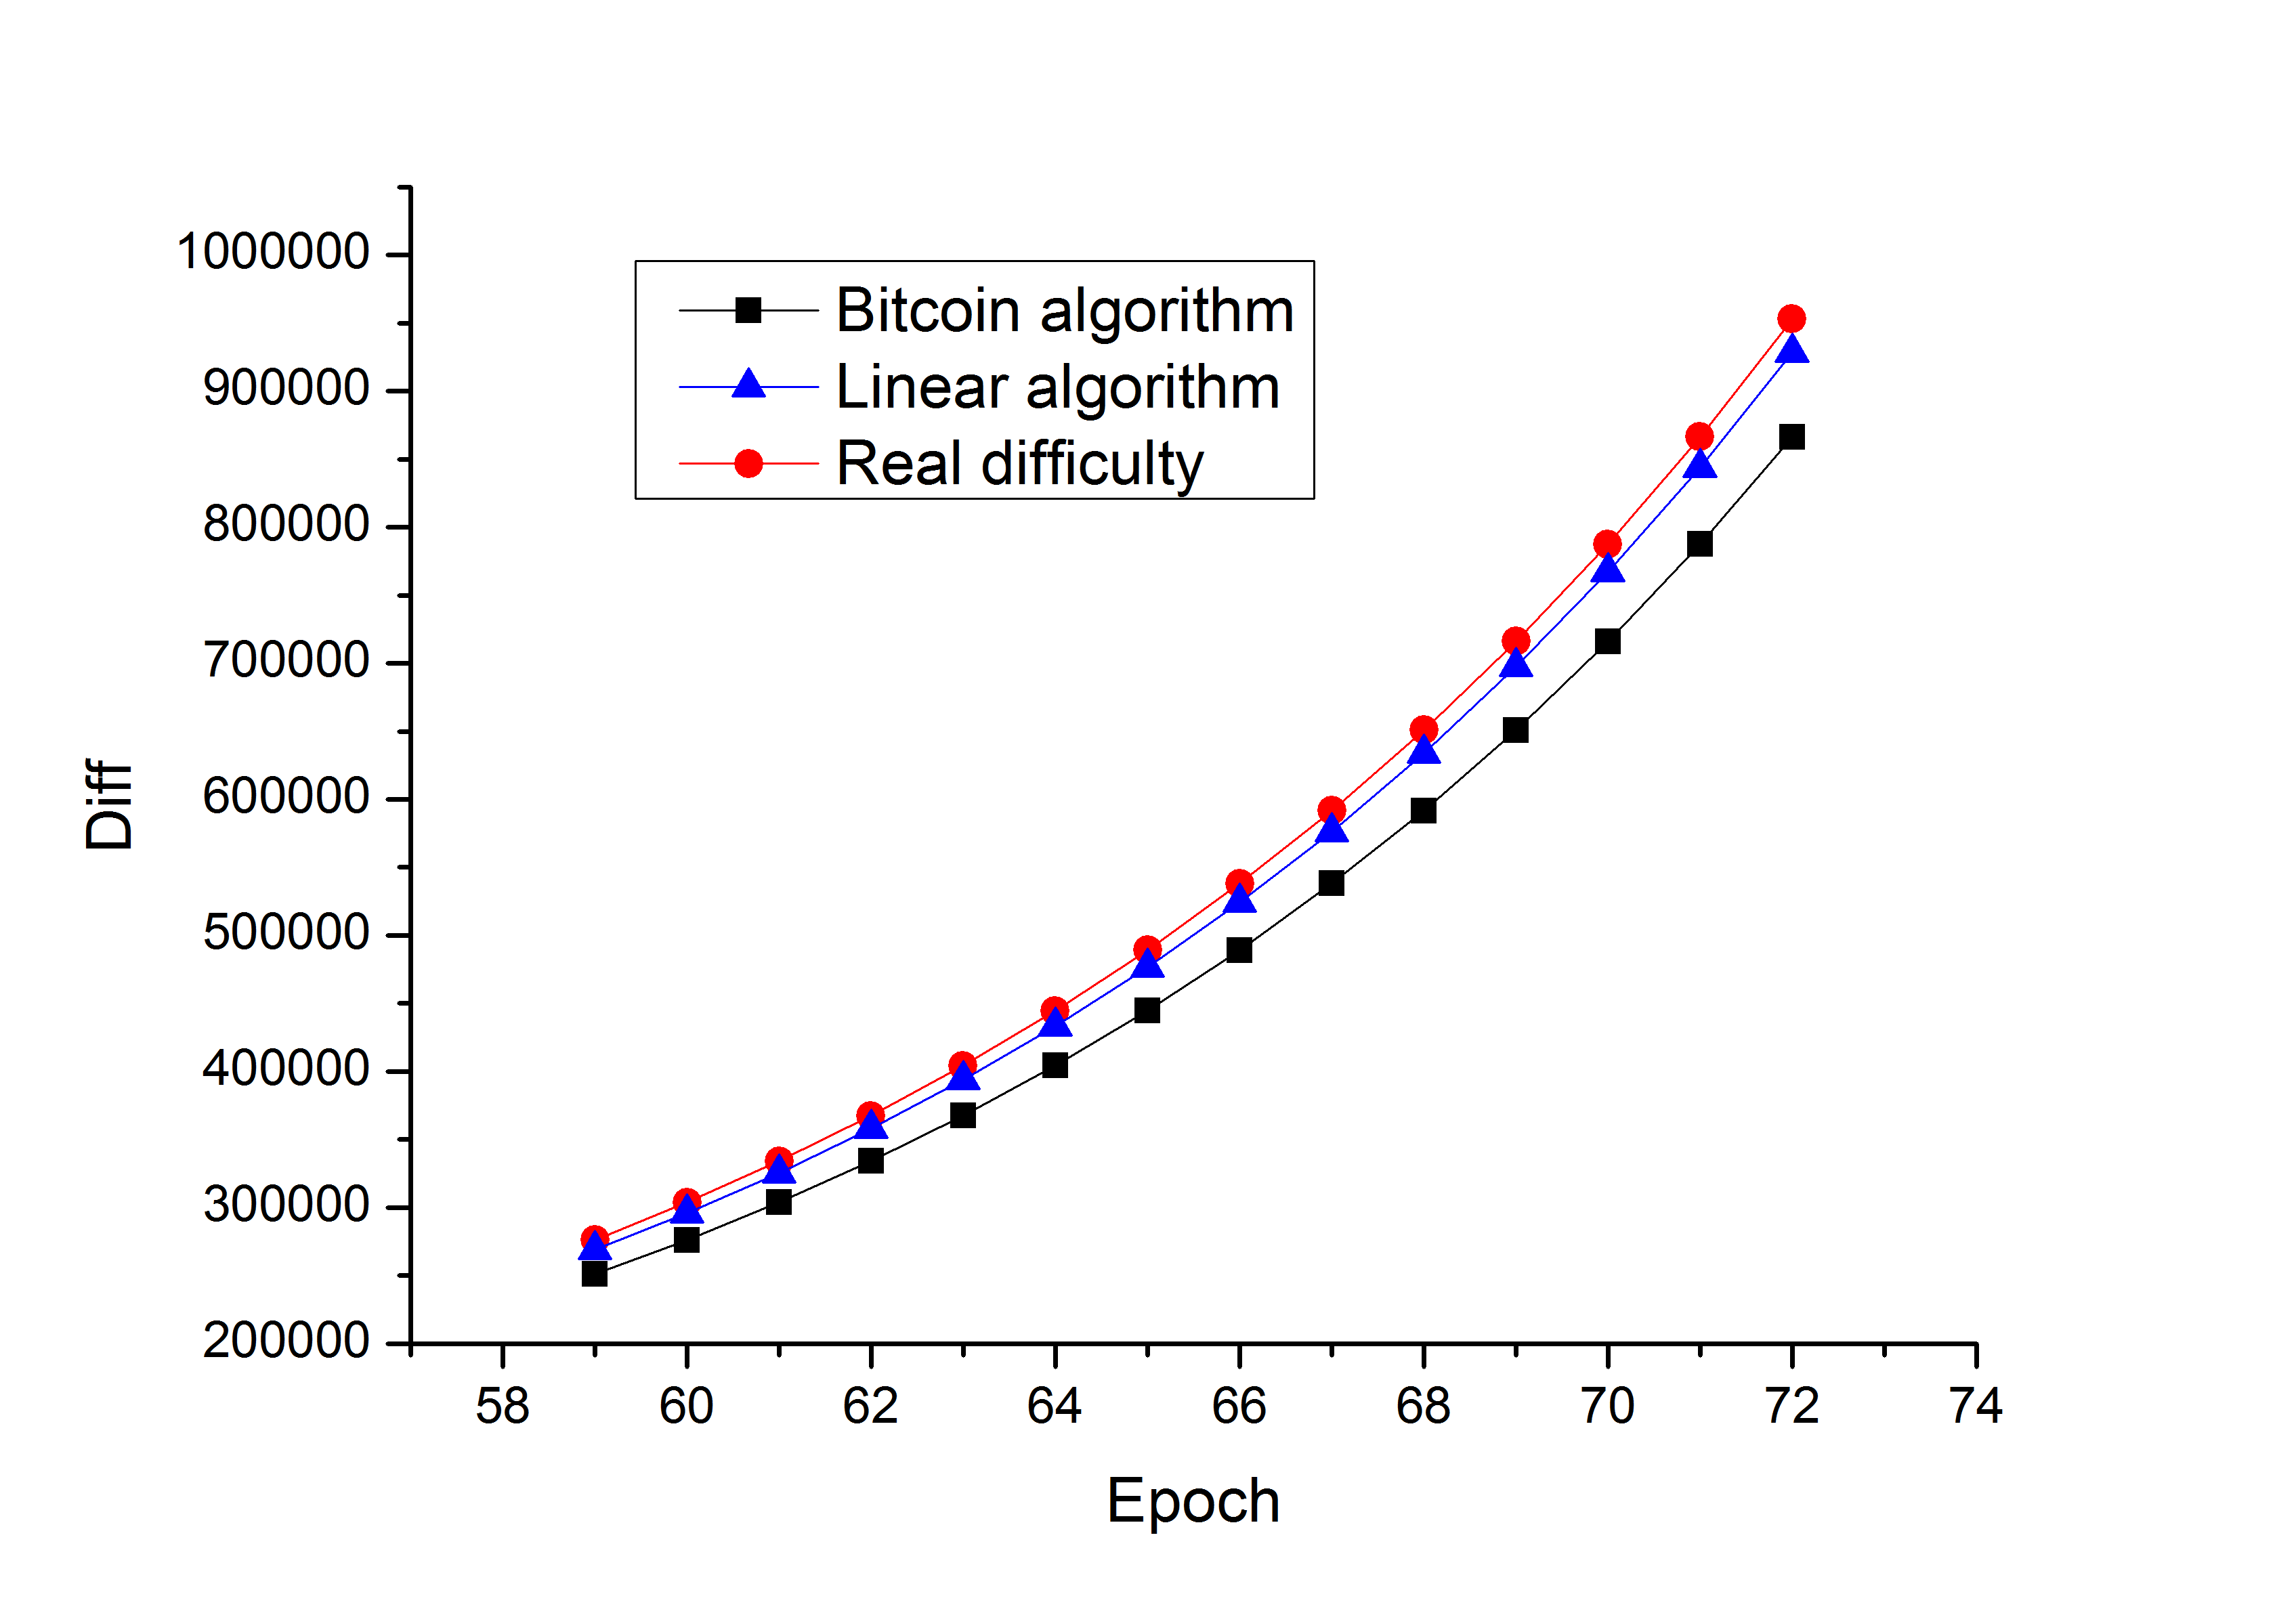
\includegraphics[scale=0.3]{exp.png}}
\caption{Real difficulty (red) and difficulties calculated from bitcoin (black) and linear (blue) algorithms in situation of exponential hash rate growth}
\label{fig:exp}
\end{figure}

Note, that difficulty, calculated from Bitcoin algorithm is always significantly lower, then the real one.
This leads to \(~ 9 min 5 sec\) time interval between blocks, which is ~10\% lower then desired \(~ 10 min\) interval.
Difficulty, calculated from Linear algorithm is also always lower, then the real one, while it's much closer to it.
Mean time interval between blocks is \(~ 9 min 45 sec\), which is much closer to the desired one.

While difficulty update algorithm, proposed in~\cite{kraft2015difficulty} leads to much better results for exponential difficulty growth with a constant rate, we should note, that our algorithm is much simplier and may be implemented with integer arithmetic only.
Moreover, exponential difficulty growth is the simplification of the difficulty growth law, and it may be incorrect to expect it in some situations.

\subsection{Fork Switch Attack}

Now let's conside a situation, regarded in Section~\ref{sec:attack}: an attacker, containing \(R_a\) computational power (for simplicity we suppose \(R_a=0.2 \cdot R_a \) in this section) turn on and turn off his mining to manipulate difficulty and minimize computational power, expended for block mining.
Figure \ref{fig:exp} represents difficulty as the function of epcoh for this situation.

\begin{figure}[h]
\center{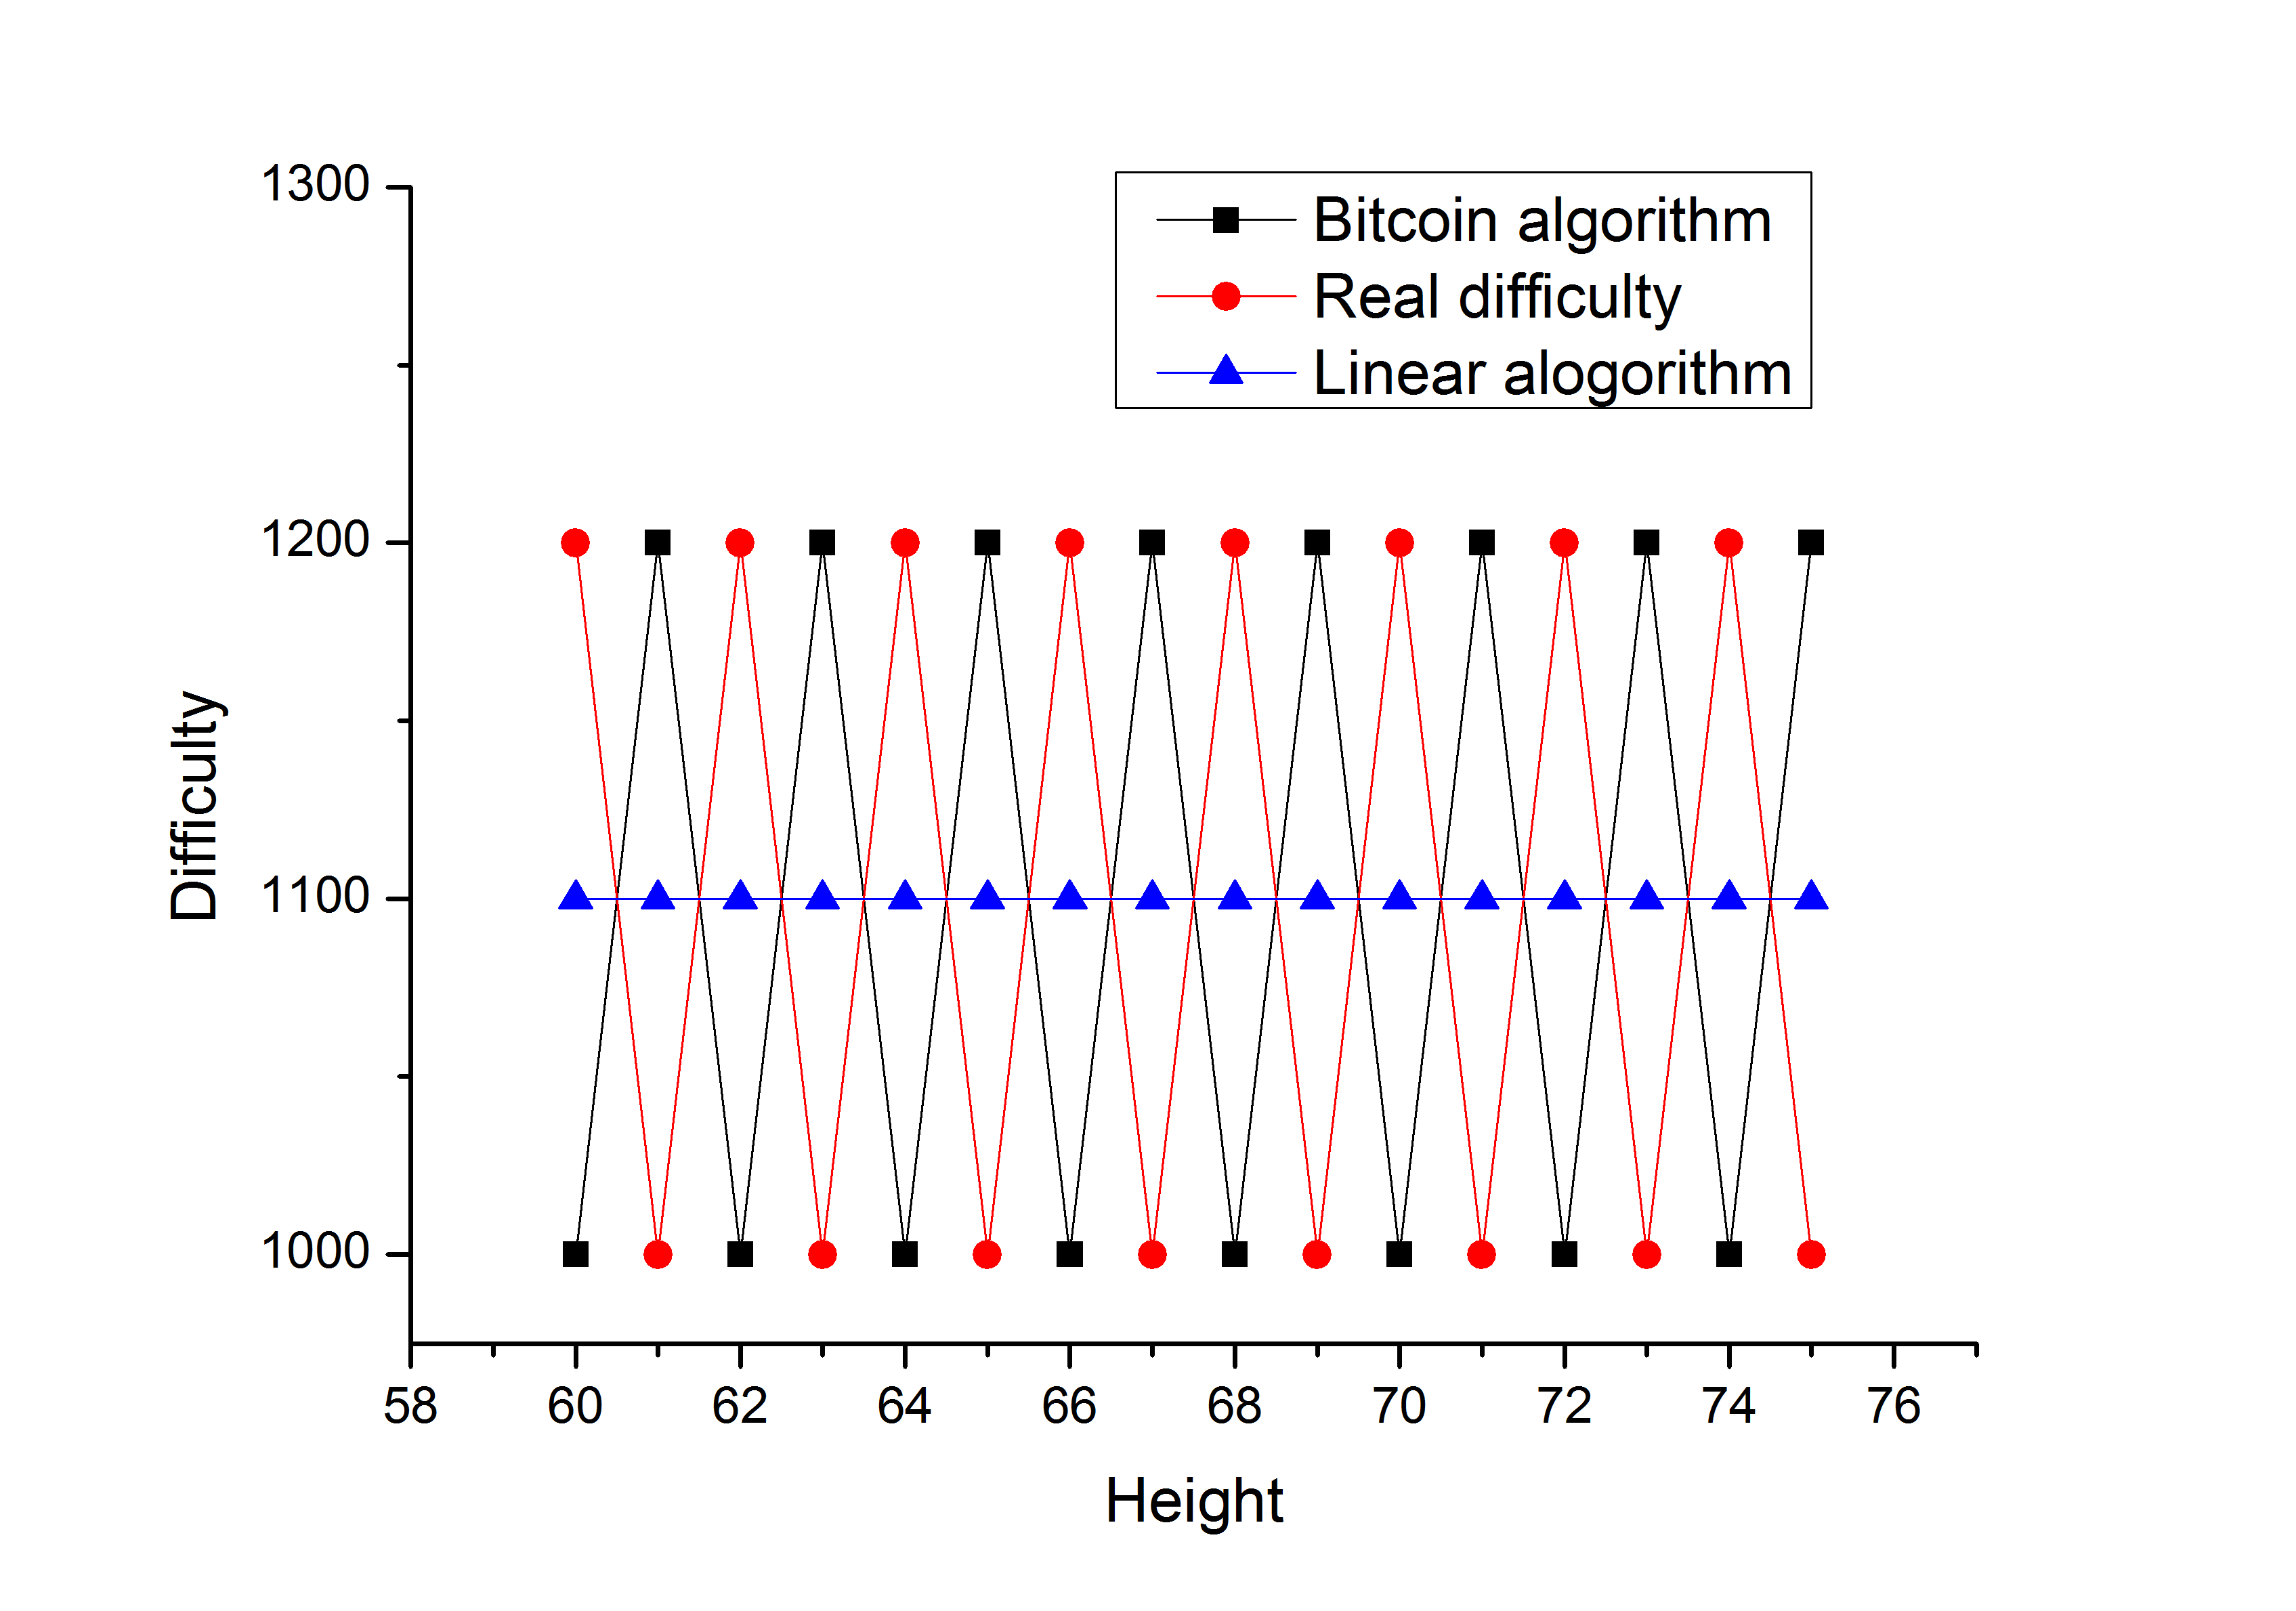
\includegraphics[scale=0.3]{attack.png}}
\caption{Real difficulty (red) and difficulties calculated from bitcoin (black) and linear (blue) algorithms in situation of attack, described in section \ref(sec:attack)}
\label{fig:attack}
\end{figure}

Note, that the difficulty, calculated from the Bitcoin algorithm is always in antiphase with the real one and the attacker spends his computational power only when difficulty is low.
Bitcoin difficulty update algorithm leads to \(~ 10 min 10 sec\) mean delay between blocks, which is in good correlation with \ref{eq:ati}.
Linear algorithm also leads to enlarged time interval between blocks  \(~ 10 min 5 sec\), but it's deviation from desired time is 2 times lower.
Obviously, attacker profit is also 2 times lower in situation with linear difficuilty update algorithm, which may be regarded as a good result.

Thus, linear difficulty control algorithm, proposed in Section \ref{sec:improved} is better, then the Bitcoin one in all situations both in terms of block rate and in terms of attacker profit.

\section{Conclusions}
\label{sec:concl}

In this paper we analyze the new way of attack on the blockchain, based on manipulating mining difficulty.
This attack decrease computational power, spended by the attacker for block mining and increase mean time interwal between blocks.
It is especially favourable in situation, when the cost of computational resourses invested into mining is around the expected reward and there are enough forks to switch mining between them.

To improve the stability of block times and decrease the attacker profit, we proposed an alternative difficulty update algorithm, based on linear regression.
It was found that this algorithm is better then the Bitcoin one both in terms of block rate and in terms of attacker profit, while it's still simple enough to be computed with integer arithmetic only.

\section*{References}

\bibliographystyle{elsarticle-num}
\bibliography{sources.bib}


\end{document}